\chapter{Theoretical part}
\section{History of virtualization}

\vspace{5mm}

While computer technology continues to march forward with smaller, sleeker, more powerful machines, in many ways how we use computers has come full circle.
Obviously the computers of today are way more powerful than the computers of the 1950s, but it turns out the way we are using them is going back to the early days 
of computing.

\vspace{5mm}

Anyone who has been around computers for a while will quickly recognize that the concept of running a client’s session on a server and then displaying the 
results on the client machine describes the way mainframes work.  Let’s take a look at the history of virtualization to see how it all began and look at some of the 
ways that the world of virtualization has evolved.

\vspace{5mm}

\section{Mainframes examples}

\vspace{5mm}
\textbf{VMware}
\vspace{5mm}
The reigning king in the world of virtualization is VMware. Their line of products (including ESX Server and VI3) has led the recent movement toward 
virtualized IT systems.

\vspace{5mm}
\textbf{Connectix Corp}
\vspace{5mm}
Connectix Corp. was a company that made virtualization software for Windows and Macintosh-based computers. In 2003 Microsoft acquired their virtualization 
technology and now uses it in their own virtualization products.

\vspace{5mm}
\textbf{Microsoft}
\vspace{5mm}
In addition to Hyper-V (the main subject of this book ), there are two other virtualization products from Microsoft out there. 
While not as grand in scope as Hyper-V, they are still a means of virtualization. Microsoft brings to the virtualization party Virtual PC, Virtual Server, and Hyper-V.

\vspace{5mm}
\section{What is Hyper-V}
\vspace{5mm}

Following the launch of Windows Server 2008, Microsoft released Windows Server 2008 Hyper-V, the hypervisor-based virtualization technology that is a role 
built into 64-bit versions of Windows Server 2008. Hyper-V offers a reliable, scalable, and high-performance virtualization platform that plugs into existing IT 
infrastructures, enabling users to consolidate some of the most demanding workloads. 

\vspace{5mm}

In addition, the Microsoft System Center product family gives customers a single 
set of integrated tools to manage physical and virtual resources, helping customers create a more agile and dynamic datacenter. Hyper-V’s scalability derives from its 
support for multiple processors and cores at the host level and improved memory limits at the host and guest level within virtual machines. This enables users to scale 
their virtualization environment to support a large number of virtual machines within a given host and to take advantage of quick migration for high availability across 
multiple hosts.

\vspace{5mm}
\section{What is a v-switch}
\vspace{5mm}

A \textbf{v-switch}, ( virtual switch more precise ), is a virtual device that give the virtual machines and the host to communicate over network.
This type of switches are completely simulating a real swithc, giving a network admin the posibility to create complex routes and networks, faster and easier that working
with physical devices. In most cases, a v-switch is used to create communication channels vetween Virtual Machines, and between virtual machines and the host.

\vspace{5mm}
\subsection{Networking options}
\vspace{5mm}

By default Hyper-V comes with three different networking settings: 
\vspace{5mm}

\begin{enumerate}
\item \textbf{External}
\item \textbf{Internal}
\item \textbf{Private} 
\end{enumerate}

\vspace{5mm}
The \textbf{External} network setting creates a connection to a physical NIC so that guest virtual machines can access the physical network to which that NIC is connected. 
\vspace{5mm}
The \textbf{Internal} setting creates a network that the host and the guest virtual machines can communicate on. 
\vspace{5mm}
The \textbf{Private} network setting creates a network that only virtual 
machines can communicate on. 
\vspace{5mm}
The main and only difference betweem Internal and Private is that the host machine does not have a NIC in the Private one. Basicly, if you add a NIC of the 
host in a Private network, it becomes an Internal one. More than likely, if you are mixing production, development, and test workloads on your virtual environments, you will have a mix 
of external, internal, and private networks.

\vspace{5mm}
\subsection{What can be filtered}
\vspace{5mm}

The Hyper-V extensible switch supports an interface that allows instances of NDIS filter drivers (known as extensible switch extensions) to bind within the extensible switch driver stack. 
After they are bound and enabled, extensions can monitor, modify, and forward packets to extensible switch ports. This also allows extensions to reject, redirect, or originate packets to 
ports that are used by the Hyper-V partitions.

\vspace{5mm}

A normal firewall, working on a machine, can have access to traffic data at the 7th from the OSI model, and more exactly at the Application Layer.
When talking about filtering traffic from a switch, the maximum layer that we can access is layer 4, and more exactly the Transport Layer.

\vspace{5mm}

The difference between the 2 aproaches is that filtring at layer 7 gives you more control over what applications access the network, or what applications
are accessed from outside the computer. Layer 7 gives us information like \textbf{Application id} and \textbf{TCP Flow Information}.

\vspace{5mm}

\begin{figure}[h]
\centering
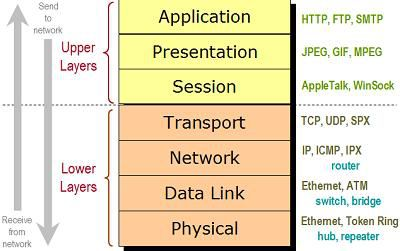
\includegraphics[width=1\textwidth]{osi-stack.jpg}
\caption{OSI Stack}
\label{osi-stack}
\end{figure}

\vspace{5mm}
\subsubsection{TCP example}
\vspace{5mm}

TCP has a well known \textit{handshake} for every connection made. It is a way to syncronize 2 endpoints and let them know how to communicate with each other.
The handshake looks like this:

\vspace{5mm}
\begin{enumerate}
\item A pachet that has \textbf{SYN} TCP flag set, is sent from the client to server.
\item A pachet that has \textbf{SYN-ACK} TCP flags set, is sent from the server to client.
\item A pachet that has \textbf{ACK} TCP flag set, is sent from the client to server.
\end{enumerate}
\vspace{5mm}

After this operation, at the operating system level, the TCP connection has been made. This connection is known as a \textbf{TCP Flow}. On a Windows machine,
the NDIS network drivers does this, with the help of tcpip.sys driver.

\vspace{5mm}

It is important to notice the fact that when working on Layer 7 as a firewall, you can detect and make a decision about every TCP Flow, without bothering with
the handshake. On the other hand, if a firewall wants to filter traffic from the siwtch, it must correlate by itself all the handhake operations to detect a TCP connection.

\vspace{5mm}
\subsubsection{Traffic directions}
\vspace{5mm}

At the machine layer, when talking about network traffic we have inbound traffic, and outbound traffic. As their name sais, inbound traffic is the one that comes from
outside and outbound traffic is the one that goes out in the network. When speaking about v-swith traffic, there is no inbound and outbound, because the refference object os not 
a machine anymore, but a switch. For these, there are the terms \textbf{Egress} and \textbf{Ingress}. \textbf{Egress} traffic is the traffic that gets out from the switch,
and \textbf{Ingress} is the traffic that goes in the switch.
\vspace{5mm}

\begin{figure}[h]
\centering
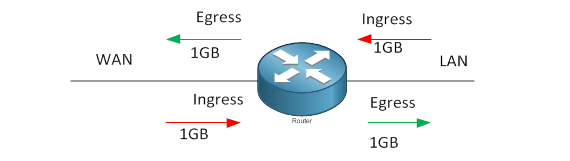
\includegraphics[width=1\textwidth]{ingress-vs-egress.png}
\caption{Ingress vs Egress direction}
\label{ingress-vs-egress}
\end{figure}

\vspace{5mm}
\section{Virtualization types}
\vspace{5mm}
There are two major types of hypervisors: a monolithic hypervisor and a microkernelized hypervisor. The monolithic hypervisor is installed directly to hardware and holds
all third-party tools and drivers required for the Admin VM and guest VMs to function. A microkernelized hypervisor, like the monolithic hypervisor, is installed directly to the
hardware but offloads driver management and the virtualization stack to the parent partition. \cite{BOOK:3}
\vspace{5mm}

\begin{figure}[h]
\centering
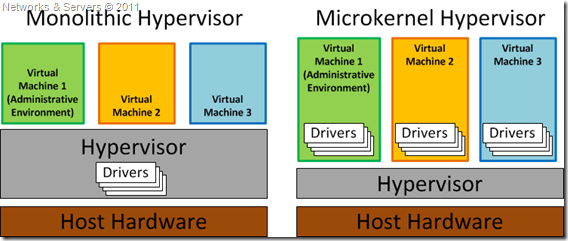
\includegraphics[width=1\textwidth]{hypervisor-types.png}
\caption{Hypervysor types}
\label{hypervisor-types}
\end{figure}

\vspace{5mm}
The Hyper-V hypervisor handles access to physical resources such as the physical processer. The hypervisor provides a virtual view of the physical components to the
partitions. Depending on the configuration, this may be a full virtual view, or the virtual view may be just a slice of the physical resources. The hypervisor uses what is called the
hypercall as the interface of communications between the partitions and the hardware. The hypervisor will also run the advanced programmable interrupt controller (APIC),
which assigns priority levels to processor interrupts. The hypervisor also manages memory address management, partitions, and memory service routines.

\vspace{5mm}
\section{Hyper-V Partitions}
\vspace{5mm}

Hyper-V creates logical units of isolation in which a guest operating system will be installed. Each of those logical units is called a partition . There are two types of 
partitions that are created in Hyper-V:
\vspace{5mm}
\begin{enumerate}
	\item the parent partition 
	\item the child partition.
\end{enumerate}

\vspace{5mm}
\subsection{Parent Partition}
\vspace{5mm}

The parent partition \cite{BOOK:1}, or root partition, runs the virtualization stack and is the partition that has direct access to the hardware devices. When you install Windows Server
2008 and then implement the Hyper-V role, your initial installation becomes the parent or root partition. The parent partition runs the virtualization service provider (VSP) that talks
directly to the device drivers through the hypervisor and offers hardware services when requested by child partitions. The virtualization stack consists of the VM worker processes,
a Windows Management Instrumentation (WMI) provider, and the VM Services. The VM worker processes are user-mode components of the virtualization stack.
The VM worker processes provide virtual machine management (VMM) services from the parent partition to the child partitions. For each child partition there is a separate set of VM worker processes created. The virtual machine management service is responsible for managing the state of each child partition.

\vspace{5mm}

The parent partition also contains a specific set of WMI APIs to allow you to programmatically control and manage a virtual machine. The virtualization infrastructure driver
(VID) and Windows Hypervisor Interface Library or WinHV components are used for physical resource management. The VID provides management services for partitions, virtual processor management, and memory management. The WinHV component allows a partitioned operating system to talk to the hypervisor directly with standard Windows calling conventions.

\vspace{5mm}

The parent partition is also used to create child partitions that will run an isolated guest operating system with applications.

\vspace{5mm}
\subsection{Child Partition}
\vspace{5mm}

The child partition \cite{BOOK:1} runs a guest operating system that can have applications installed and running many different functions of a business. If a supported hypervisoraware operating system is installed on the guest virtual machine or child partition, it will run the virtualization service client or VSC. The VSC consumes the services that the VSP makes available for use.

\vspace{5mm}

Hyper-V categorizes operating systems into two different categories:
\vspace{5mm}
\begin{enumerate}
	\item hypervisoraware operating system 
	\item non-hypervisor-aware operating system
\end{enumerate}

\vspace{5mm}

A hypervisoraware operating system is extremely similar to a paravirtualized operating system.

\vspace{5mm}

Paravirtualization is a method that lets a guest operating system know that it’s being virtualized and allows for the host system and the guest system to cooperate to help
reduce the performance cost on key functions of a guest operating system. Hypervisoraware operating systems work directly with Hyper-V to realize performance and management gains by taking advantage of Enlightened I/O.

\vspace{5mm}

Two different types of devices are present in a child partition:
\vspace{5mm}
\begin{enumerate}
	\item synthetic
	\item emulated
\end{enumerate}

\vspace{5mm}
A \textbf{synthetic} device is designed to have the lowest overhead and utilizes the VMBUS to send packaged instructions to a driver on the parent partition

\vspace{5mm}
An \textbf{emulated} device is a device that emulates a physical device such as a network interface card. After you install a supported operating system onto a child partition, 
you will want to install the integration components on that operating system. Integration components are a set of services and drivers that help the virtual machine perform and behave 
in a more consistent manner. There are integration components for both Windows and Linux operating systems. The Windows Integration Components installs the virtualization service client 
as well as time synchronization, heartbeat, shutdown, key/value pair exchange, and the Volume Shadow Copy Service (VSS).

\vspace{5mm}
The time synchronization component plays an important role in keeping child partitions in sync. This can be achieved using a network protocol as well, but the time synchronization component comes in handy when a network resource isn’t available, or where a network protocol may be too slow. Having the ability to synchronize time quickly becomes
very important when restoring a virtual machine from a saved state, or when bringing a virtual machine back online that has been in a dormant state for an extended period of time.

\vspace{5mm}
The parent partition will use the heartbeat component to send a regular request to the child partition to verify if that partition is available. If the parent partition doesn’t
receive a response in a timely manner, it will continue to request a status and will log
events for the missing replies.

\vspace{5mm}
\subsection{VMBus}
\vspace{5mm}

The virtual machine bus (VMBUS) \cite{BOOK:2} is used for communication between the parent and child partition via the virtual service provider and the virtual service client. The VMBUS
provides a virtualized environment if your system is running a virtualization-optimized processor.

\vspace{5mm}
\section{Windows Kernel}
\vspace{5mm}

To protect user applications from accessing and/or modifying critical operating system data, Windows
uses two processor access modes (even if the processor on which Windows is running supports more
than two): user mode and kernel mode \cite{BOOK:1} . User application code runs in user mode, whereas operating
system code (such as system services and device drivers) runs in kernel mode. Kernel mode refers to
a mode of execution in a processor that grants access to all system memory and all CPU instructions.
By providing the operating system software with a higher privilege level than the application software
has, the processor provides a necessary foundation for operating system designers to ensure that a
misbehaving application can’t disrupt the stability of the system as a whole.

\vspace{5mm}
\section{Network drivers}
\vspace{5mm}

Network drivers take high-level I/O requests and translate them into low-level network protocol
requests for transmission across the network. The network APIs rely on transport protocol drivers in
kernel mode to perform the actual translation. Separating APIs from underlying protocols gives the
networking architecture the flexibility of letting each API use a number of different protocols.

\vspace{5mm}
\subsection{Windows Filtering Platform}
\vspace{5mm}

Windows Filtering Platform (WFP) is a set of API and system services that provide a platform for creating network filtering applications. The WFP API allows developers to write code that interacts with the packet processing that takes place at several layers in the networking stack of the operating system. Network data can be filtered and also modified before it reaches its destination.

\vspace{5mm}
\cite{BOOK:1} Windows includes a rich and extensible platform for monitoring, intercepting, and processing
network traffic at all levels in the network stack. Other Windows networking services extend basic
networking features of the TCP/IP protocol driver by relying on Windows Filtering Platform (WFP).
These include Network Address Translation (NAT), IP filtering, IP inspection, and Internet Protocol
Security (IPsec).

\vspace{5mm}

With the WFP API, developers can implement firewalls, intrusion detection systems, antivirus programs, network monitoring tools, and parental controls. The WFP API consists of a user-mode API and a kernel-mode API.

\vspace{5mm}

Some of the major component of WFP are:
\vspace{5mm}
\begin{enumerate}

\item Filter engine. The filter engine is implemented in both user mode and kernel mode and performs all the filtering operations on the network. Each filter engine component consists of
filtering layers, one for each component of the network stack.

\item Shims. Shims are the kernel-mode components that reside between the network stack and the filter engine. They are responsible for making the decision to allow or block network traffic
based on their filtering behavior, which is defined by the filter engine. A shim operates in three steps: it parses the incoming data to match incoming values with entries in the filter engine,
calls the filter engine to return an action based on the incoming values, and then interprets the action (drop the packet, for example).

\item Base filtering engine (BFE). The BFE is a user-mode service that manages all WFP operations. It is responsible for adding and removing filters from the WFP stack, managing the filter 
configuration, and enforcing security on the filter database.

\item Callout drivers. Callout drivers are kernel-mode components that add custom filtering functionality outside the basic support provided by the WFP. Callout drivers associate callout 
functions with one or more kernel-mode filtering layers, and the WFP enables callout functions to perform deep packet inspection and modification. This topic will be the most covered in the
upcoming details.

\end{enumerate}

\vspace{5mm}

\subsubsection{Filters}

\vspace{5mm}
The main functionality of WFP is the filter registration. A filter is basicaly a set of conditions that tells the WFP whether or not to match a certain traffic. For example a filter can contain the condition of \textbf{remote port 80}, and will match only the traffic that goes to or comes from port 80. The matching action is defined by the developer and it can mainly be to block or allow the traffic, but we will talk about this later.

\vspace{5mm}
Each filter can have a \textbf{weight} that represents its order in the filter stack. A filter with a higher weight has priority over others with lower weights. This mechanism allow for complex scenarios and customizations of a network filtering application.
Here is an example of 2 rules, given in the order of their priorities ( high to low ):
\vspace{5mm}
\begin{enumerate}
\item Allow port 80
\item Block ( all )
\end{enumerate}

\vspace{5mm}
In the above example we allowed for port 80, which means that all connection to port 80 will pass, while others will be blocket. If the block rule had a higher weight, it would have blocked all traffic, including port 80.

\vspace{5mm}
There are 2 types of filters:
\vspace{5mm}

\begin{enumerate}
\item Action filters
\item Callout filters
\end{enumerate}

\vspace{5mm}
An action filter has 2 possible verdicts: allow and block. This is usualy used in simple firewall rules when someone knows exatly what needs to be filtered and the conditions provided by WFP cover them all ( will talk about conditions soon ).
\vspace{5mm}

A callout filter is a filter that has a callout attached to it for better detections, filtering and complex logic. Sometimes one does not have all the conditions for filtering given by WFP, and needs to register a callout in order to filter the traffic based on more criterias.  In most cases, a filtering traffic utility does that, like a parental control product. It has to register callouts in order to access the data received on that connection, parse it and see if there is anything suspicious or matches a product policy and then take the action of blocking of permiting the traffic. 

\vspace{5mm}
\subsubsection{Filter Arbitration Behaviors}
\vspace{5mm}

Filter arbitration is the logic built into the Windows Filtering Platform (WFP) that is used to determine how filters interact with each other when making network traffic filtering decisions.

\vspace{5mm}
The following behaviors characterize the filter arbitration system:
\vspace{5mm}

\begin{enumerate}
\item All traffic can be inspected. No traffic can bypass filters at a given layer.
\item Traffic can be blocked by a callout filter via a Veto even if a higher priority filter has permitted it.
\item Multiple providers can inspect traffic at the same layer. For example, firewall followed by intrusion-detection system (IDS) filters, or IPsec followed by Quality of Service (QoS) filters may all examine the traffic at the same layer.
\end{enumerate}
\vspace{5mm}

Within a sub-layer, filter arbitration is performed as follows:

\vspace{5mm}
\begin{enumerate}
\item Compute the list of matching filters ordered by weight from highest to lowest.
\item Evaluate matching filters in order until a "Permit" or a "Block" is returned (filters can also return "Continue") or until the list is exhausted.
\item Skip the remaining filters and return the action from the last evaluated filter.
\end{enumerate}

\vspace{5mm}
Within a layer, filter arbitration is performed as follows:
\vspace{5mm}

\begin{enumerate}
\item Perform filter arbitration at every sub-layer in order from highest priority to lowest priority.
\item Evaluate all sub-layers even if a higher priority sub-layer has decided to block the traffic.
\item Return the resulting action based on the policy rules described in the following section.
\end{enumerate}

\vspace{5mm}

\subsubsection{Application Programming Interface}

\vspace{5mm}

The following function is used to add a filter to WFP engine.
\vspace{5mm}
\begin{lstlisting}
DWORD FwpmFilterAdd0(
  HANDLE               		engineHandle,
  const FWPM_FILTER0   	*filter,
  PSECURITY_DESCRIPTOR sd,
  UINT64               		*id
);
\end{lstlisting}
\vspace{5mm}

The handle to the filter engine is received after a call \textbf{FwpmEngineOpen0} to open a session.

\vspace{5mm}

This is the filter object structure. There are multiple fields that tell the filter where it must apply, and fileds that tell the filter how to behave.

\vspace{5mm}
\begin{lstlisting}
typedef struct FWPM_FILTER0_ {
  GUID                   	filterKey;
  FWPM_DISPLAY_DATA0     	displayData;
  UINT32                 	flags;
  GUID                   	*providerKey;
  FWP_BYTE_BLOB          	providerData;
  GUID                   	layerKey;
  GUID                   	subLayerKey;
  FWP_VALUE0                weight;
  UINT32                 	numFilterConditions;
  FWPM_FILTER_CONDITION0 	*filterCondition;
  FWPM_ACTION0              action;
  union {
    UINT64 rawContext;
    GUID   providerContextKey;
  };
  GUID                   	*reserved;
  UINT64                 	filterId;
  FWP_VALUE0             	effectiveWeight;
} FWPM_FILTER0;
\end{lstlisting}
\vspace{5mm}

The above are just some example in order to make a better idea about the functionality. Please go to the official documentation from Microsoft for a full documentation and explication.

\vspace{5mm}
\subsubsection{Layer available for filtering}
\vspace{5mm}

WFP lets a developer choose at which layer the traffic should be filtered.

\vspace{5mm}

The Windows Filtering Platform (WFP) layer identifiers are each represented by a GUID.
For example \textbf{FWPM LAYER ALE AUTH LISTEN V4} layer allows for authorizing TCP listen requests. Looking again at the above example with port 80, if the filter is at this layer the rule will match only if it is an inbound connection to the local machine. A connection from the local machine to a server will not trigger the rule. 

\vspace{5mm}

There are a lot of layers available for filtering coresponding to the OSI model and more, but the ones we are interested in in this article are the following: 

\vspace{5mm}
\begin{enumerate}
\item FWPS\_LAYER\_INGRESS\_VSWITCH\_ETHERNET
\item FWPS\_LAYER\_EGRESS\_VSWITCH\_ETHERNET
\item FWPS\_LAYER\_INGRESS\_VSWITCH\_TRANSPORT\_V4
\item FWPS\_LAYER\_INGRESS\_VSWITCH\_TRANSPORT\_V6
\item FWPS\_LAYER\_EGRESS\_VSWITCH\_TRANSPORT\_V4
\item FWPS\_LAYER\_EGRESS\_VSWITCH\_TRANSPORT\_V6
\end{enumerate}
\vspace{5mm}

\subsubsection{Filtering conditions}
\vspace{5mm}

Filter conditions are entities that help a developer vary the rules applied to the network stack.

\vspace{5mm}

\begin{lstlisting}
typedef struct FWPM_FILTER_CONDITION0_ {
  GUID                 fieldKey;
  FWP_MATCH_TYPE       matchType;
  FWP_CONDITION_VALUE0 conditionValue;
} FWPM_FILTER_CONDITION0;
\end{lstlisting}

\vspace{5mm}

This is the layout of a condition. There must be an array of them applied to the \textbf{filterCondition} field of the \textbf{FWPM\_FILTER0}. ALso it is mandatory to set the counter to the proper value.

\vspace{5mm}

The conditions are valuated in the order in which they are inserted in the array. If every condition matches the traffic, the filter will match and apply the verdict or call the callout. 

\vspace{5mm}

As an example, we can have the following conditions: \textbf{port 80} and \textbf{application == chrome.exe}. Wfp applies this filters over all traffic, and if and only if the traffic is from \textbf{Chrome.exe} and on \textbf{port 80} it will apply the action.

\vspace{5mm}

There is a special rule in the implementation of WFP condition checking. If there are multiple consecutive conditions of the same type ( let's say port conditions ) , WFP will apply an \textbf{AND} between them, otherwise an \textbf{AND}. For a better overview let's take the above example but add
a new port conditons. This time we have \textbf{port 443} , \textbf{port 80} and \textbf{application == chrome.exe}. In this case, the formula for checking if the traffic matches the rule is:
\vspace{5mm}

\begin{lstlisting}
port 443 OR port 80 AND Chrome.exe.
\end{lstlisting}

\vspace{5mm}
As you can see, if there are multiple conditions of the same type, but not consecutive in the array, the filter might not match any traffic. If the evaluation is done this way : 
\vspace{5mm}

\begin{lstlisting}
port 443 AND Chrome.exe OR port 80.
\end{lstlisting}

\vspace{5mm}
WFP will not match any traffic due to the fact that there cannot be traffic on both ports 443 and 80 in the same time. ( talking about remote ports here ).
\vspace{5mm}

The Windows Filtering Platform (WFP) filter engine supports a different set of filtering conditions at each of its filtering layers.

\vspace{5mm}

\textbf{The layers are: }
\vspace{5mm}
\begin{enumerate}
\item FWPM\_LAYER\_EGRESS\_VSWITCH\_TRANSPORT\_V4
\item FWPM\_LAYER\_INGRESS\_VSWITCH\_TRANSPORT\_V4
\item FWPM\_LAYER\_INGRESS\_VSWITCH\_TRANSPORT\_V6
\item FWPM\_LAYER\_EGRESSVSWITCH\_TRANSPORT\_V6
\end{enumerate}
\vspace{5mm}
\textbf{The conditions available are:}
\vspace{5mm}
\begin{enumerate}
\item FWPM\_CONDITION\_IP\_SOURCE\_ADDRESS
The source ip of the ip header
\item FWPM\_CONDITION\_IP\_DESTINATION\_ADDRESS
The destination ip of the ip header
\item FWPM\_CONDITION\_IP\_PROTOCOL
The protocol from the ip header ( tcp, udp, icmp )
\item FWPM\_CONDITION\_IP\_SOURCE\_PORT
The source port of the transport header ( tcp port or udp port )
\item FWPM\_CONDITION\_IP\_DESTINATION\_PORT
The destination port of the transport header ( tcp port or udp port )
\item FWPM\_CONDITION\_VLAN\_ID
\item FWPM\_CONDITION\_VSWITCH\_TENANT\_NETWORK\_ID
\item FWPM\_CONDITION\_VSWITCH\_ID
\item FWPM\_CONDITION\_VSWITCH\_NETWORK\_TYPE
\item FWPM\_CONDITION\_VSWITCH\_SOURCE\_INTERFACE\_ID
\item FWPM\_CONDITION\_VSWITCH\_SOURCE\_INTERFACE\_TYPE
\item FWPM\_CONDITION\_VSWITCH\_SOURCE\_VM\_ID
The id of the source VM. This is is represented by a GUID.
\item FWPM\_CONDITION\_VSWITCH\_DESTINATION\_INTERFACE\_ID
\item FWPM\_CONDITION\_VSWITCH\_DESTINATION\_INTERFACE\_TYPE
\item FWPM\_CONDITION\_VSWITCH\_L2\_FLAGS
Layer 2 flags represent the type of layer 2 protocol, as ARP, IP, etc
\end{enumerate}

\vspace{5mm}
\subsubsection{Callouts}
\vspace{5mm}

The filter engine calls a callout's classifyFn callout function when there is network data to be processed by the callout. This occurs when all the filtering conditions are true for a filter that specifies the callout for the filter's action. If such a filter has no filtering conditions, the filter engine always calls the callout's classifyFn callout function.

\vspace{5mm}

The filter engine passes several different data items to a callout's classifyFn callout function. These data items include fixed data values, metadata values, raw network data, filter information, and any flow context. The particular data items that the filter engine passes to the callout depend on the specific filtering layer and the conditions 
under which classifyFn is called. A classifyFn function can use any combination of these data items to make its filtering decisions.

\vspace{5mm}

The following function is the prototype of the function that needs to be implemented by a developer in order to access and modify a network packet. In this callout a packet can be pended 
( pend the operation ) and after all the processing has been made the operation can be completed and the pended packet reinjected in the network stack ( with or without changes from the
original format ) 

\vspace{5mm}

\begin{lstlisting}
VOID NTAPI ClassifyFn(
    IN const FWPS_INCOMING_VALUES0  *inFixedValues,
    IN const FWPS_INCOMING_METADATA_VALUES0  *inMetaValues,
    IN OUT VOID  *layerData,
    IN const FWPS_FILTER0  *filter,
    IN UINT64  flowContext,
    IN OUT FWPS_CLASSIFY_OUT0  *classifyOut
    );
\end{lstlisting}

\vspace{5mm}

This is this callout registration structure. One must fill this structure with all the information needed by WFP in order for it to work properly. The \textbf{ClassifyFn} function pointer
must point to a function as described above. It will be called every time the filter containing this callout matches a traffic packet and will be called with it as the \textbf{layerData}
parameter.

\vspace{5mm}

\begin{lstlisting}
const FWPS_CALLOUT0 Callout =
{
 { ... }, // GUID key identifying the callout
 0,       // Callout-specific flags (none set here)
 ClassifyFn,
 NotifyFn,
 FlowDeleteFn
};
\end{lstlisting}

\vspace{5mm}

Here is an example of how a callout is registered in the system. Firstly, for the WFP to know about filters and their coresponding identifiers ( GUIDS ), the callout must be registered first 
before it is used. After the callout is registered, it can be used in the filter registration by its GUID.

\vspace{5mm}

\begin{lstlisting}
NTSTATUS DriverEntry(
    IN PDRIVER_OBJECT DriverObject,
    IN PUNICODE_STRING RegistryPath
    )
{
  PDEVICE_OBJECT deviceObject;
  NTSTATUS status;

  ...

 status =
 FwpsCalloutRegister0(
 deviceObject,
      &Callout,
      &CalloutId
      );
\end{lstlisting}

\vspace{5mm}

\subsubsection{IRQL}

\vspace{5mm}

IRQL stands for \textbf{Interrupt Request Level}.

\vspace{5mm}

The priority ranking of an interrupt. A processor has an IRQL setting that threads can raise or lower. Interrupts that occur at or below the processor's IRQL setting are masked and will 
not interfere with the current operation. Interrupts that occur above the processor's IRQL setting take precedence over the current operation.

\vspace{5mm}

The particular IRQL at which a piece of kernel-mode code executes determines its hardware priority. Kernel-mode code is always interruptible: an interrupt with a higher IRQL value can 
occur at any time, thereby causing another piece of kernel-mode code with the system-assigned higher IRQL to be run immediately on that processor. In other words, when a piece of code 
runs at a given IRQL, the Kernel masks off all interrupt vectors with a lesser or equal IRQL value on the microprocessor.

\vspace{5mm}

\begin{figure}[h]
\centering
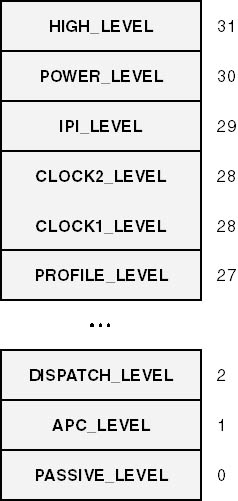
\includegraphics[]{IRQL.jpg}
\caption{IRQL}
\label{IRQL}
\end{figure}

\vspace{5mm}

The User Mode processes run at passive level. That is why even if a process hangs, the mouse can still be moved, due to the fact that the interupt for the mouse has a higher priority.

\vspace{5mm}

The WFP callouts are usually called at \textbf{DISPATCH\_LEVEL}. The interesting thing about this level is that the windows thread scheduler works at the same IRQL. As the theory sais
that only a higher ( not equal ) IRQL can interupt other ones, it is self explanatory that if a thread at DISPATCH\_LEVEL is blocked, the hole system is blocked ( excepting things like the clock,
POWER, etc ).

\vspace{5mm}

If a thread stays too much at DISPATCH\_LEVEL windows will trigger a Blue Screen of Death. More exactly, this BSOD is caused by a windows component named \textbf{Watchdog timer} which checks
if threads stay too much acumulated time on DISPATCH\_LEVEL, or too much time at once.

\vspace{5mm}

Threads cand raise or lower their IRQL by calling \textbf{KeLowerIrql} and \textbf{KeRaiseIrql}